%%%%%%%%%%%%%%%%%%%%%%%%%%%%%%%%%%%%%%%%%
% Beamer Presentation
% LaTeX Template
% Version 1.0 (10/11/12)
%
% This template has been downloaded from:
% http://www.LaTeXTemplates.com
%
% License:
% CC BY-NC-SA 3.0 (http://creativecommons.org/licenses/by-nc-sa/3.0/)
%
%%%%%%%%%%%%%%%%%%%%%%%%%%%%%%%%%%%%%%%%%

%----------------------------------------------------------------------------------------
%   PACKAGES AND THEMES
%----------------------------------------------------------------------------------------

\documentclass{beamer}

\mode<presentation> {

% The Beamer class comes with a number of default slide themes
% which change the colors and layouts of slides. Below this is a list
% of all the themes, uncomment each in turn to see what they look like.

%\usetheme{default}
%\usetheme{AnnArbor}
%\usetheme{Antibes}
%\usetheme{Bergen}
%\usetheme{Berkeley}
%\usetheme{Berlin}
%\usetheme{Boadilla}
%\usetheme{CambridgeUS}
%\usetheme{Copenhagen}
%\usetheme{Darmstadt}
%\usetheme{Dresden}
%\usetheme{Frankfurt}
%\usetheme{Goettingen}
%\usetheme{Hannover}
%\usetheme{Ilmenau}
%\usetheme{JuanLesPins}
%\usetheme{Luebeck}
\usetheme{Madrid}
%\usetheme{Malmoe}
%\usetheme{Marburg}
%\usetheme{Montpellier}
%\usetheme{PaloAlto}
%\usetheme{Pittsburgh}
%\usetheme{Rochester}
%\usetheme{Singapore}
%\usetheme{Szeged}
%\usetheme{Warsaw}

% As well as themes, the Beamer class has a number of color themes
% for any slide theme. Uncomment each of these in turn to see how it
% changes the colors of your current slide theme.

%\usecolortheme{albatross}
%\usecolortheme{beaver}
%\usecolortheme{beetle}
%\usecolortheme{crane}
%\usecolortheme{dolphin}
%\usecolortheme{dove}
%\usecolortheme{fly}
%\usecolortheme{lily}
%\usecolortheme{orchid}
%\usecolortheme{rose}
%\usecolortheme{seagull}
%\usecolortheme{seahorse}
%\usecolortheme{whale}
%\usecolortheme{wolverine}

%\setbeamertemplate{footline} % To remove the footer line in all slides uncomment this line
%\setbeamertemplate{footline}[page number] % To replace the footer line in all slides with a simple slide count uncomment this line

%\setbeamertemplate{navigation symbols}{} % To remove the navigation symbols from the bottom of all slides uncomment this line
}

\usepackage{graphicx} % Allows including images
\usepackage{booktabs} % Allows the use of \toprule, \midrule and \bottomrule in tables

\usepackage[utf8x]{inputenc} %%  toto je pre citanie slovenskych symbolov
\usepackage[slovak]{babel}   %%  aj toto :)
%\usepackage[english]{babel}   %%  aj toto :)
\usepackage{xcolor}

\usepackage[T1]{fontenc}
\usepackage{graphicx}

\usepackage{comment}

%----------------------------------------------------------------------------------------
%   TITLE PAGE
%----------------------------------------------------------------------------------------

%\title[JPEG Steganography]{Image-based steganography using mobile app} % The short title appears at the bottom of every slide, the full title is only on the title page
\title[JPEG Steganografia]{Android aplikácia pre obrázkovú steganografiu} % The short title appears at the bottom of every slide, the full title is only on the title page


\author{Askar Gafurov} % Your name
\institute[FMFI UK] % Your institution as it will appear on the bottom of every slide, may be shorthand to save space
{
%Faculty of mathematics, physics and informatics \\ % Your institution for the title page
%Comenius University in Bratislava \\
Fakulta matematiky, fyziky a informatiky\\
Univerzita Komenského v Bratislave \\
\medskip
\url{ksp.sk/~askar} % Your email address
}
\date{13. júna 2016} % Date, can be changed to a custom date

\begin{document}

\begin{frame}
\titlepage % Print the title page as the first slide
\end{frame}


\begin{frame}
\frametitle{Čo je steganografia?}
\begin{block}{}
\textit{Steganografia} je umenie skrytej komunikácie.

%\end{block}
%\begin{block}{}
Na rozdiel od kryptografie, je potrebné ukryť nie obsah správy, ale samotnú jej \textit{pritomnosť}.
\end{block}

\begin{block}{}
\textit{Steganalýza} je komplementárna oblasť, ktorá sa zaoberá odhaľovaním skrytých správ.
    
\end{block}

\begin{figure}

\includegraphics[height=0.2\textheight]{images/stegosaurus.png}
\end{figure}
\end{frame}

\begin{frame}
    \frametitle{Vývoj steganografie}
    \begin{block}{Minulosť}
        Triky, chémia, fyzika
        \begin{itemize}
            \item Neviditeľný atrament
            \item Mikrobodky v nenápadných pohľadniciach
            \item Správy vytetované na hlavách otrokov
        \end{itemize}
    \end{block}
    \begin{block}{Súčasnosť --- digitálna éra}
        Matematika
        \begin{itemize}
            \item Vkládanie správ do digitálnych médií: obrázky, videá, hudba
        \end{itemize}
    \end{block}
\end{frame}


\begin{frame}
    \frametitle{Príklad}
    \begin{figure}
    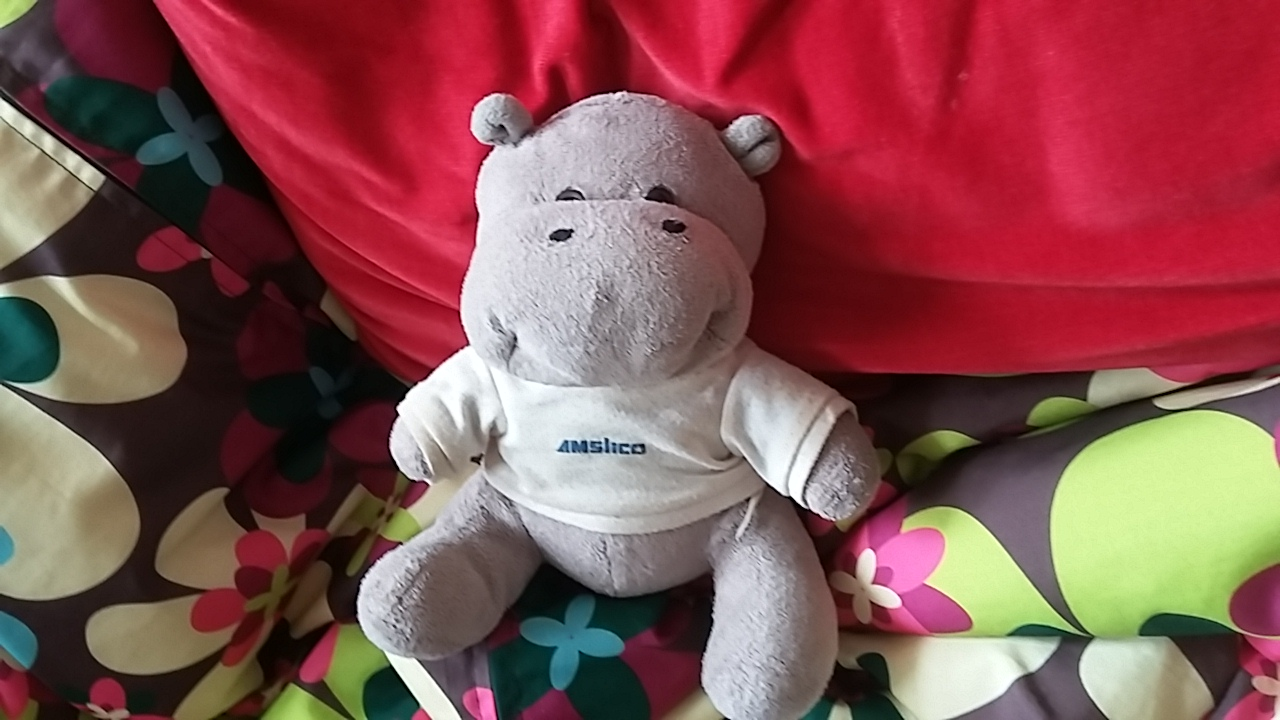
\includegraphics[height=0.4\textheight]{images/original.jpg}
    \end{figure}
    \begin{figure}
    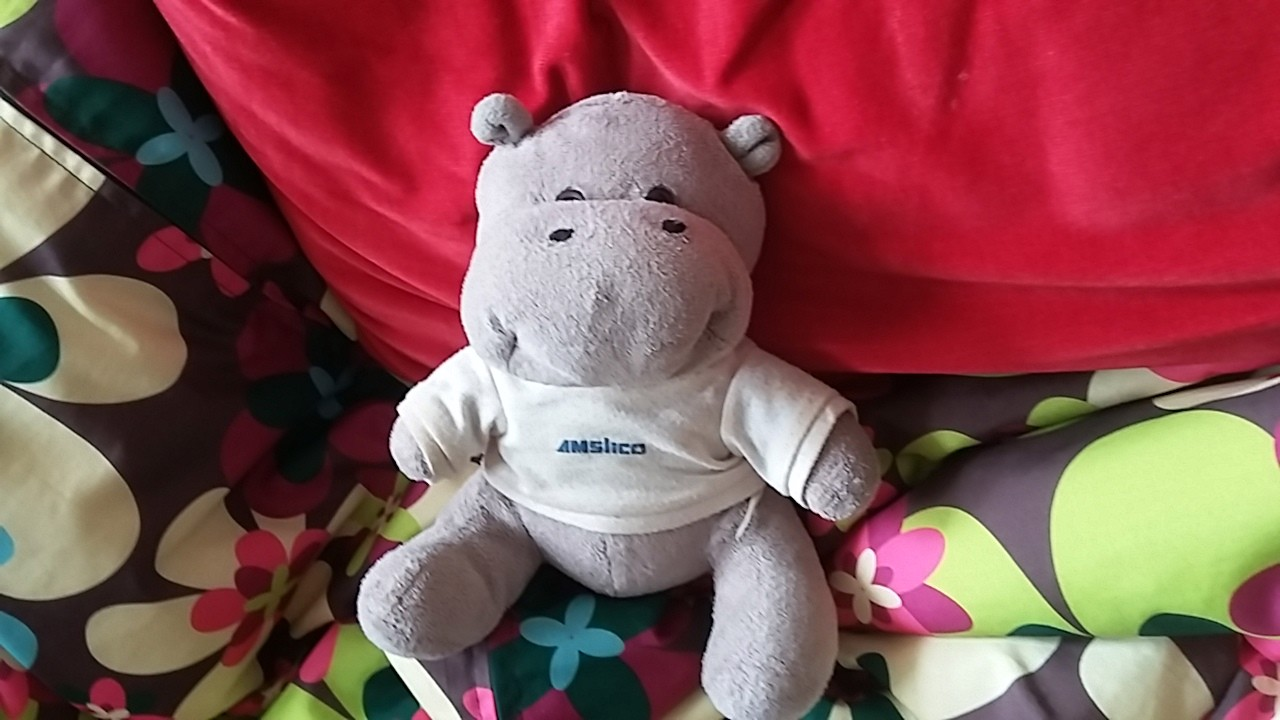
\includegraphics[height=0.4\textheight]{images/embedded.jpg}
    \end{figure}
    
\end{frame}

% 
% \begin{frame}
%      \frametitle{Súčasný stav digitálnej steganografie}
%      \begin{block}{}
%          \begin{itemize}
%              \item Nové algoritmy a metódy vznikajú každý rok
%              \item Narastá komplexnosť riešení 
%              \item Bezplatný softvér je vo veľmi zlom stave 
%          \end{itemize}
%     \end{block}
% \end{frame}
% 
% aby sme vobec rozumeli ze co chceme

% \begin{frame}
%     \frametitle{JPEG ako prenosové médium}
%     \begin{block}{JPEG kompresia}
%         \begin{itemize}
%             \item Transformation from RGB to YCbCr color space
%             \item Reduction of Cb and Cr channels definition (lossy operation)
%             \item Splitting each channel into $8 \times 8$ bytes long blocks 
%             \item Discrete cosine transformation (DCT) of numbers in each block
%             \item Rounding of DCT coefficients (main lossy operation)
%             \item (Lossless) compression of coefficients (main compression operation)
%         \end{itemize}
%     \end{block}
%     \begin{block}{}
%         \textbf{Obrázok sa dá vnímať ako zoznam bytov --- \textit{koeficientov~DCT}}
%     \end{block}
% \end{frame}

\begin{frame}
    \frametitle{Moderné metódy}
    \begin{itemize}
        \item prvá metóda: \emph{Least Significant Bits (LSB)}
        \item prvý útok založený na štatistike: \emph{chi-square} (1999)
        \item algoritmy F5, Outguess (2001)
        \item S-rodina útokov (2002)
        \item útoky na základe strojového učenia (SVM) (2002)
        \item komplementárne vkládanie (2008)
        \item nový prístup: genetické algoritmy (2009)
        \item použitie štat. vlastností Fourierovej transformácie,\\
            Benfordov zákon (2013)
    \end{itemize}
\end{frame}

\begin{frame}
    \frametitle{Problémy súčasných aplikácií}
    \begin{itemize}
        \item Skrytá implementácia
        \item Neznáme a/alebo zastaralé algoritmy
        \item Nespravné použitie algoritmov
        \item Neohraničená dĺžka správ
        \item Žiadne požiadavky na silu kľúčov, prípadne totálna absencia kľúčov
        \item Použivanie bezstratových formátov
        \item Podpora iba ASCII symbolov
        \item Žiadna kompresia a/alebo kryptografia
        \item Dovolené opätovné použitie krycích obrázkov
    \end{itemize}
\end{frame}

\begin{frame}
    \frametitle{Návrh špecifikácie}
    \begin{itemize}
        \item Moderné algoritmy
        \item Povinná komprimácia a šifrovanie posielanej správy
        \item Závislosť na kľúčoch + manažement kľúčov
        \item Optimálne podmienky neodhaliteľnosti
        \item Podpora UTF-8
        \item Vymeniteľnosť použitých algoritmov
        \item Otvorený kód
    \end{itemize}
    
\end{frame}

\begin{frame}
    \frametitle{Schéma vkládania a extrákcie}
    % pregenerovany pomocou dia (polozka pixbuf[png])
    \begin{figure}
    %vlozenie samotneho obrazku vycentrovaneho a vhodnej velkosti
    %obrazok je v subore images/cervik.png
    \centerline{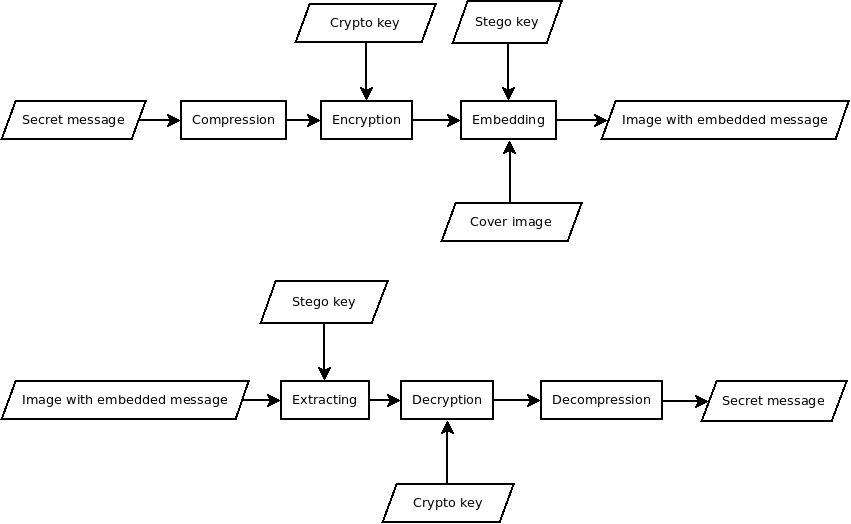
\includegraphics[width=\textwidth]{diagrams/flow.png}}
    %popis obrazku
    %\caption[Main pipelines]{Main pipelines. Upper part: embedding process, lower part: extracting process}
    %id obrazku, pomocou ktoreho sa budeme na obrazok odvolavat
    \label{img:CSflow}
    \end{figure}
    
\end{frame}

\begin{frame}
    \frametitle{Použité algoritmy}
    \begin{itemize}
        \item Steganografia --- komplementárne vkládanie
        \item Kryptográfia --- AES-256
        \item Kompresia --- GZIP
    \end{itemize}
    
\end{frame}

\begin{frame}
    \frametitle{Optimálne podmienky použitia}
    \begin{itemize}
        \item Nepouživajte dvakrát ten istý obrázok
        \item Neposielajte dvakrát tú istú správu
        \item Použivajte rôznorodé farebné obrázky
        \item Často meňte svoje kľúče
        \item Generujte svoje kľúče pomocou bezpečných mechanizmov
        \item Použivajte bezpečné kanály na distribúciu kľúčov
        \item Posielajte čo najkratšie správy
    \end{itemize}
\end{frame}


\begin{frame}
    \frametitle{Výsledky práce}
    \begin{itemize}
        \item Prehľad moderných metód
        \item Zoznam chýb a špecifikácia, ktorá ich eliminuje
        \item Návrh metódy na použivanie stratových kanálov
        \item Implementovaná modulárna open-source aplikácia
        \item Voľne dostupna Java implementácia novšieho rýchleho steganografického algoritmu (lepší ako F5)
        \item Odhalená chyba v originálnom článku (podrobnejšie v texte práce)
    \end{itemize}
    
\end{frame}


\begin{frame}
    \frametitle{Budúca práca}
    \begin{itemize}
        \item Prídanie asymetrického šifrovania
        \item Pokročilý manažement kľúčov (potrebný pre asym. šifrovanie)
        \item Krajšie použivateľské rozhranie
        \item Odolnosť voči dodatočnej kompresii obrázkov
        \item Prídanie vstavaných testov pomocou známych steganalýtických nástrojov
    \end{itemize}
    
\end{frame}

\begin{frame}
    \begin{center}
        \Large Ďakujem za pozornosť!
    \end{center}
\end{frame}

\begin{frame}
    \begin{center}
        \Large
        Otázky?
    \end{center}
\end{frame}

\section{Technické detaily}

\section{Úkažka}

\section{Budúca práca}


\begin{comment}
\section{What is steganography?}
\begin{frame}
\frametitle{What is steganography?}
\pause
No, it's not "writing about stegosaurs" :) 
\begin{figure}

\includegraphics[height=0.5\textheight]{images/stegosaurus.png}
\end{figure}
\end{frame}

\begin{frame}
\frametitle{What is steganography?}

\begin{block}{}
\emph{It's the art of covered or hidden writing.}    
\end{block}

\end{frame}

\section{Image-based steganography}
\subsection{How it should work}
\begin{frame}
\frametitle{How it should work}
    \begin{enumerate}
        \item Alice takes a photo of her delicious double decaf latte with pumpkin flavour
        \item Alice types hidden message to it (a la tweet :) )
        \item Alice posts image with injected text e.g. on facebook
        \pause
        \item Bob downloads Alice's posted photo
        \item Bob types password to unlock hidden content of image
        \item Bob reads hidden message
    \end{enumerate}
\end{frame}

\subsection{Lossless formats: Least significat bits}
\begin{frame}
\frametitle{How to inject message into PNG image?}
\begin{itemize}
    \item PNG image is a bunch of pixels
    \item Each pixel is encoded by 3 numbers (RGB model)
    \pause
    \item we can change last bits of each pixel to match our message\ldots
    \pause
    but it would be too obvious 
    \pause
    \item correction: using secret stego-key choose random pixels to inject bits of secret message
    \item decoding is simple: using same secret stego-key determine which pixels have been chosen to inject data,
        and extract last bits of them 
\end{itemize}
\end{frame}

\begin{frame}
    \frametitle{Problems?}
    \begin{block}{}
        \Large No one use lossless formats to send photos over Internet.
    \end{block}
    \begin{block}{}
        Therefore, if you use lossless format, you become suspicious.
    \end{block}
\end{frame}

\subsection{Lossy formats}
\begin{frame}
\frametitle{How to inject message into JPEG image?}
\begin{block}{What is an JPEG image?}
JPEG encoding process which comprises
three major steps: forward DCT (FDCT), quantization, and entropy
encoding. The input image is first divided into $8 \times 8$
non-overlapping blocks, and each block is transformed by the
FDCT into a set of 64 DCT coefficients. These coefficients are
then 
% quantized using a quantization table with 64 entries. The
% quantized results are all integers and defined as the division of
% each DCT coefficient by its corresponding quantization value,
% and rounding to the nearest integer.
% 
bla bla bla \ldots
\end{block}
\pause
\begin{block}{for those who don't like long texts\ldots}
Output of JPEG compression is a bunch of numbers (so called \emph{DCT coefficients}).
\pause {\color{red} We can use previous method!}
\end{block}
\end{frame}

\section{Problem: Steganalysis}
\begin{frame}
    \frametitle{Problem: Steganalysis}
    \begin{block}{}
        Steganalysis is the art of revealing hidden messages :)
        
        \pause
        \medskip 
        Unfortunately, nowadays it usually comes with lots of \emph{beautiful math}
    \end{block}
    
\end{frame}

\section{Plan}

\begin{frame}
\frametitle{Plan}
\begin{block}{}
    \begin{enumerate}
        \item Producing a sufficient overview of related topics in image-based steganography.
        \item Producing a sufficient overview of applications similar to the intended one, analyzing their advantages and disadvantages.
        \item Performing a requirements engineering phase, identifying key requirements and security concerns.
        \item Designing, developing, and documenting the resulting application.
    \end{enumerate}
\end{block}
    
\end{frame}

\section{Outro}
\begin{frame}
    \begin{center}
    \Large So long and thanks for all the fish!
    \begin{figure}
        \includegraphics[height=0.5\textheight]{images/dolphins.jpg}
    \end{figure}
    \end{center}
    
\end{frame}

\begin{frame}
    \begin{center}
        \Large Questions?
    \end{center}
\end{frame}
\end{comment}
\end{document} 
